\section{Preliminaries}
\subsection{Definitions}
%A graph is a 2-tuple consisting of a vertex set and an edge set. The visualization, however, has to be drawn in some kind of way. Investigating the drawing of a graph needs to include several constraints, for example, \textit{how} we want the drawing and \textit{where} we want to draw on. These constraints can be described mathematically.\\
As otherwise mentioned, a \textit{graph} $G=(V_G,E_G)$ is a tuple consisting of two sets - the set of vertices and the set of edges. An \textit{edge} $e = (v,w), v,w \in V_G$ is a tuple and describes a connectivity relation between two vertices. Unless otherwise mentioned, the graphs are \textit{undirected}. It means that the edge $(u,v)$ is identical to the edge $(v,u)$,$u,v\in V_G$. A \textit{face} is a maximal open region of the plane bounded by edges. The \textit{degree} of a vertex states the amount of edges incident to the vertex. The \textit{degree} of a graph $G$ is the maximum of the degree of its vertices. A \textit{drawing} $\Gamma$ of a graph $G$ is a function, where each vertex is mapped on a unique point $\Gamma(v)$ in the plane and each edge is mapped on an open Jordan curve $\Gamma(e)$ ending in its vertices. A graph is \textit{planar} if and only if there exists a crossing-free representation in the plane. An \textit{embedding} of $G$ is the collection of counter-clockwise circular orderings of edges around each vertex of $V_G$. \cite[p.225]{Ortho}
\\
In the following sections, $G$ will be a planar undirected simple graph. $k$-planarity will refer to a planar graph with maximum degree $k$. We will now define the distinctive layouts of graphs.
\begin{definition}[Line drawings]
	A straight line drawing is a drawing where every edge is drawn as a straight line. In a polyline drawing, each edge is represented by a non-empty sequence of line segments ($e = (e_1,e_2,...)$), where two consecutive line segments intersect in a unique point. The complexity of an edge is the length of its line segment sequence.
\end{definition}
\begin{definition}[Bends]
	A \textit{bend} describes the orientation of two segments. A \textit{right bend} is defined by a 90\degree~angle in counter-clockwise direction, whereas a \textit{left bend} is defined by a 270\degree~angle respectively.
\end{definition}
\begin{definition}[Polyedge]
	A \textit{polyedge} is a sequence of edge segments such that two consecutive segments meet in a single point in the drawing.
\end{definition}
\begin{definition}
	A polyedge is called uniform if and only if all bends are of the same direction. Similarily, a polyedge is alternating if and only if all bends are alternating (staircase).\label{def:uni_alt}
\end{definition}
\begin{definition}[Orthogonal drawings, {\cite[p. 225]{Ortho}}]
	An orthogonal drawing of a graph is a polyline drawing where every edge consists of polyline segments in alternating horizontal and vertical direction. It is clear that all bends are right or left bends, as defined before.
\end{definition}
\begin{definition}[Ports]
	A \textit{port} of a vertex in an orthogonal drawing describes the position, where the edges are connected to. Due to the fact that every edge of an orthogonal drawing consists of horizontal and vertical segments, there are four ports per vertex in total for each of the cardinal directions.
\end{definition}
One of the most fundamental models is the so-called \textit{Kandinsky model}. It is a well-established and widely used graph-drawing model. It contains a \textit{grid embedding}, where a grid is used to draw the polyedges and vertices as boxes.
\begin{definition}[Kandinsky, {\cite{GD95}}]
	A Kandinsky drawing $\Gamma(G)$ of a graph with arbitrary maximum degree is an orthogonal drawing of a graph $G$ on a grid embedding. This model inherits
	\begin{itemize}
		\item a coarse grid for the vertices which is a subset of a fine grid for the edges. The granularity of the fine grid is determined by the maximum degree of $G$;
		\item every vertex is illustrated as a box with a uniform size centered on the coarse grid;
		\item every edge is drawn as a sequence of alternating horizontal and vertical line segments;
		\item there are as many edges per vertex side possible as the maximum degree of $G$ specifies.
	\end{itemize}
\end{definition}
\begin{figure}[H]
	\centering
	\begin{subfigure}{0.3\textwidth}
		\centering
		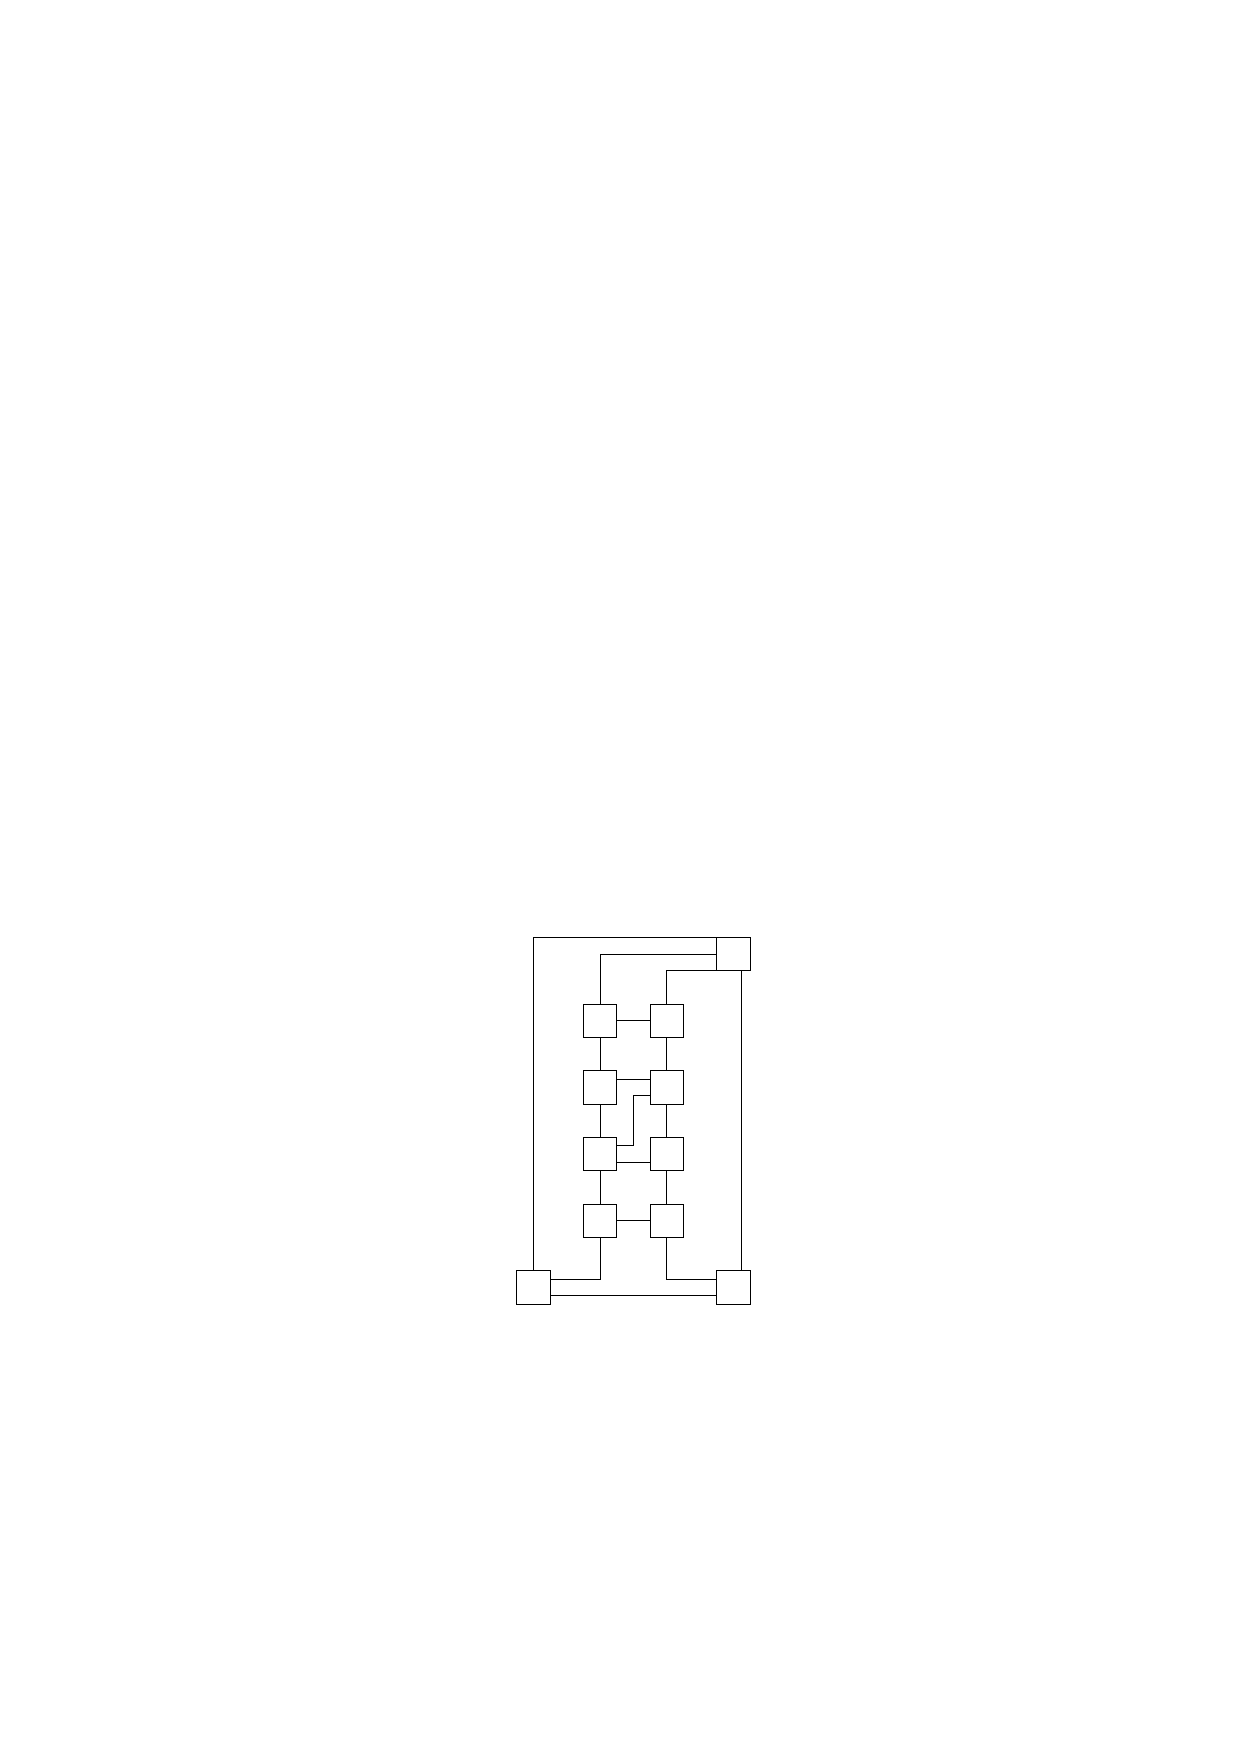
\includegraphics[width=0.6\linewidth,page=1]{includegraphics/big-example}
	\end{subfigure}
	\caption{An example for a Kandinsky drawing}
\end{figure}
A face is \textit{empty}, if for each vertex defining the face, the corresponding edges are connected to the same port. See Figure \ref{im:empty_T} for the empty $T$-face. 
\begin{figure}[H]
	\centering
	\begin{subfigure}{0.4\textwidth}
		\centering
		\includegraphics[width=0.34\linewidth,page=6]{includegraphics/L-t-shape_candidates}
		\caption{Empty $T$-face}\label{im:empty_T}	
\end{subfigure}
	\begin{subfigure}{0.4\textwidth}
		\centering
		\includegraphics[width=0.6\linewidth,page=2]{includegraphics/L-t-shape_candidates}
		\caption{Almost empty $T$-face}\label{im:almost_empty_T}
	\end{subfigure}
	\caption{Introducing diagonal line segments, empty faces can be avoided in a drawing}
\end{figure}
Those empty faces are generally forbidden in the Kandinsky model, as they imply computational errors. In order to avoid empty faces, the model is slightly altered by introducing diagonal line segments resulting in drawings with so-called \textit{almost empty} faces (See Figure \ref{im:almost_empty_T}).
\begin{definition}[Podevsaef drawings, {\cite{podevsaef}}]
	A \textit{Planar Orthogonal Drawing With Equal Vertex Size and Almost-Empty faces} (\textit{Podevsaef drawing} in short) is a drawing in which:
	\begin{itemize}
		\item The vertices are mapped on a point in the plane underlying a coarse grid and are illustrated with a uniform box,
		\item the polyedges are illustrated in the plane as a sequence of horizonal, diagonal and vertical line segments,
		\item arbitrary many edge segments can be connected to one port of the vertex box (usually, the degree of the graph as an upper bound),
		\item the diagonal segment is of length at most third of the length of the unit of the coarse grid and is never incident to a vertex box,
		\item the minimum of the angles formed by two consecutive segments of the edge is always 135\degree.
	\end{itemize}\label{def:podevsaef}
\end{definition}
\begin{figure}[H]
	\centering
	\begin{subfigure}{0.3\textwidth}
		\centering
		\includegraphics[width=0.6\linewidth,page=6]{includegraphics/big-example}
	\end{subfigure}
	\caption{An example for a podevsaef drawing}
\end{figure}
\subsection{Plane Sweep Algorithm}
The plane sweep algorithm is a procedure to gain information or even modify the drawing of a graph. The main components are a \textit{sweep line}, which iterates over a drawing in a desired direction and a data structure for so-called \textit{events}. The sweep line recognizes predefined conditions as events and saves them in the \textit{event holder}. The data structure used for storing the events is a balanced tree in standard practice in order to guarantee an appropriate runtime regarding deletion, insertion and update functions. It may be used to determine the number of crossing line segments or even alter the shape of a given drawing, as we will see with the stretching technique.
\subsection{4M Algorithm {\cite{4M}}}\label{section:4M}
Orthogonal drawing algorithms may output drawings with many bends and a large area. The 4M Algorithm addresses the quality improvement of orthogonal graph drawings. Mainly, there are four operations given by the algorithm - \textit{Moving, Matching, Morphing} and \textit{Merging}. The input drawing $\Gamma$ is preprocessed to $\Gamma ''$, before any of those algorithms work on them. At first, crossings and bends are substituted with a vertex rectangle, then horizontal stripes, creating not necessarily bounded rectangles, are introduced. The reason for this preprocessing is to avoid overlapping parts in the resulting drawing. For this thesis, the \textit{Moving} algorithm may be of interest. \textit{Matching}, \textit{Morphing} and \textit{Merging} operations may actively alter the size of the vertex boxes and are therefore not part of this thesis.
\subsubsection*{The Model}
The drawing plane is subdivided by horizontal and vertical gridlines of a unit spacing $\lambda$. The vertices are represented by rectangles of size $\left(w\lambda - \frac{\lambda}{2}\right)\times\left(h\lambda - \frac{\lambda}{2}\right);w,h\in\mathbb{N}_+$. Those rectangles overlap the grid lines by $\frac{\lambda}{4}$. 
\subsubsection*{Moving}
Finding a moving line is the first step for area savings. In order to save in horizontal area, the moving line is set vertically from top to bottom in the drawing. For vertical area savings, define the moving line similarly from left to right in the drawing.
\begin{definition}[Moving line $J$]
	An area-saving moving line $J$ is a line that fulfills the following conditions:
	\begin{itemize}
		\item $J$ is directed and consists of horizontal and vertical segments
		\item $J$ starts above the topmost object of $\Gamma ''$ and ends below the bottommost object of $\Gamma ''$
		\item $J$ does not intersect any vertical edge of $\Gamma ''$
		\item Every horizontal edge of $\Gamma ''$ that is intersected by a piece of $J$ which is directed downward has a finite length larger than or equal to two.
	\end{itemize}
\end{definition}
Once $J$ is found, we can reduce the length of the segments crossed downwards and lengthening the segments crossed upwards consecutively by one unit until one of the segments is reduced up to the unit length. Since $J$ intersects the border of $\Gamma''$ in downward direction, the total area decreases.
\begin{figure}[H]
	\centering
	\begin{subfigure}{0.4\textwidth}
		\centering
		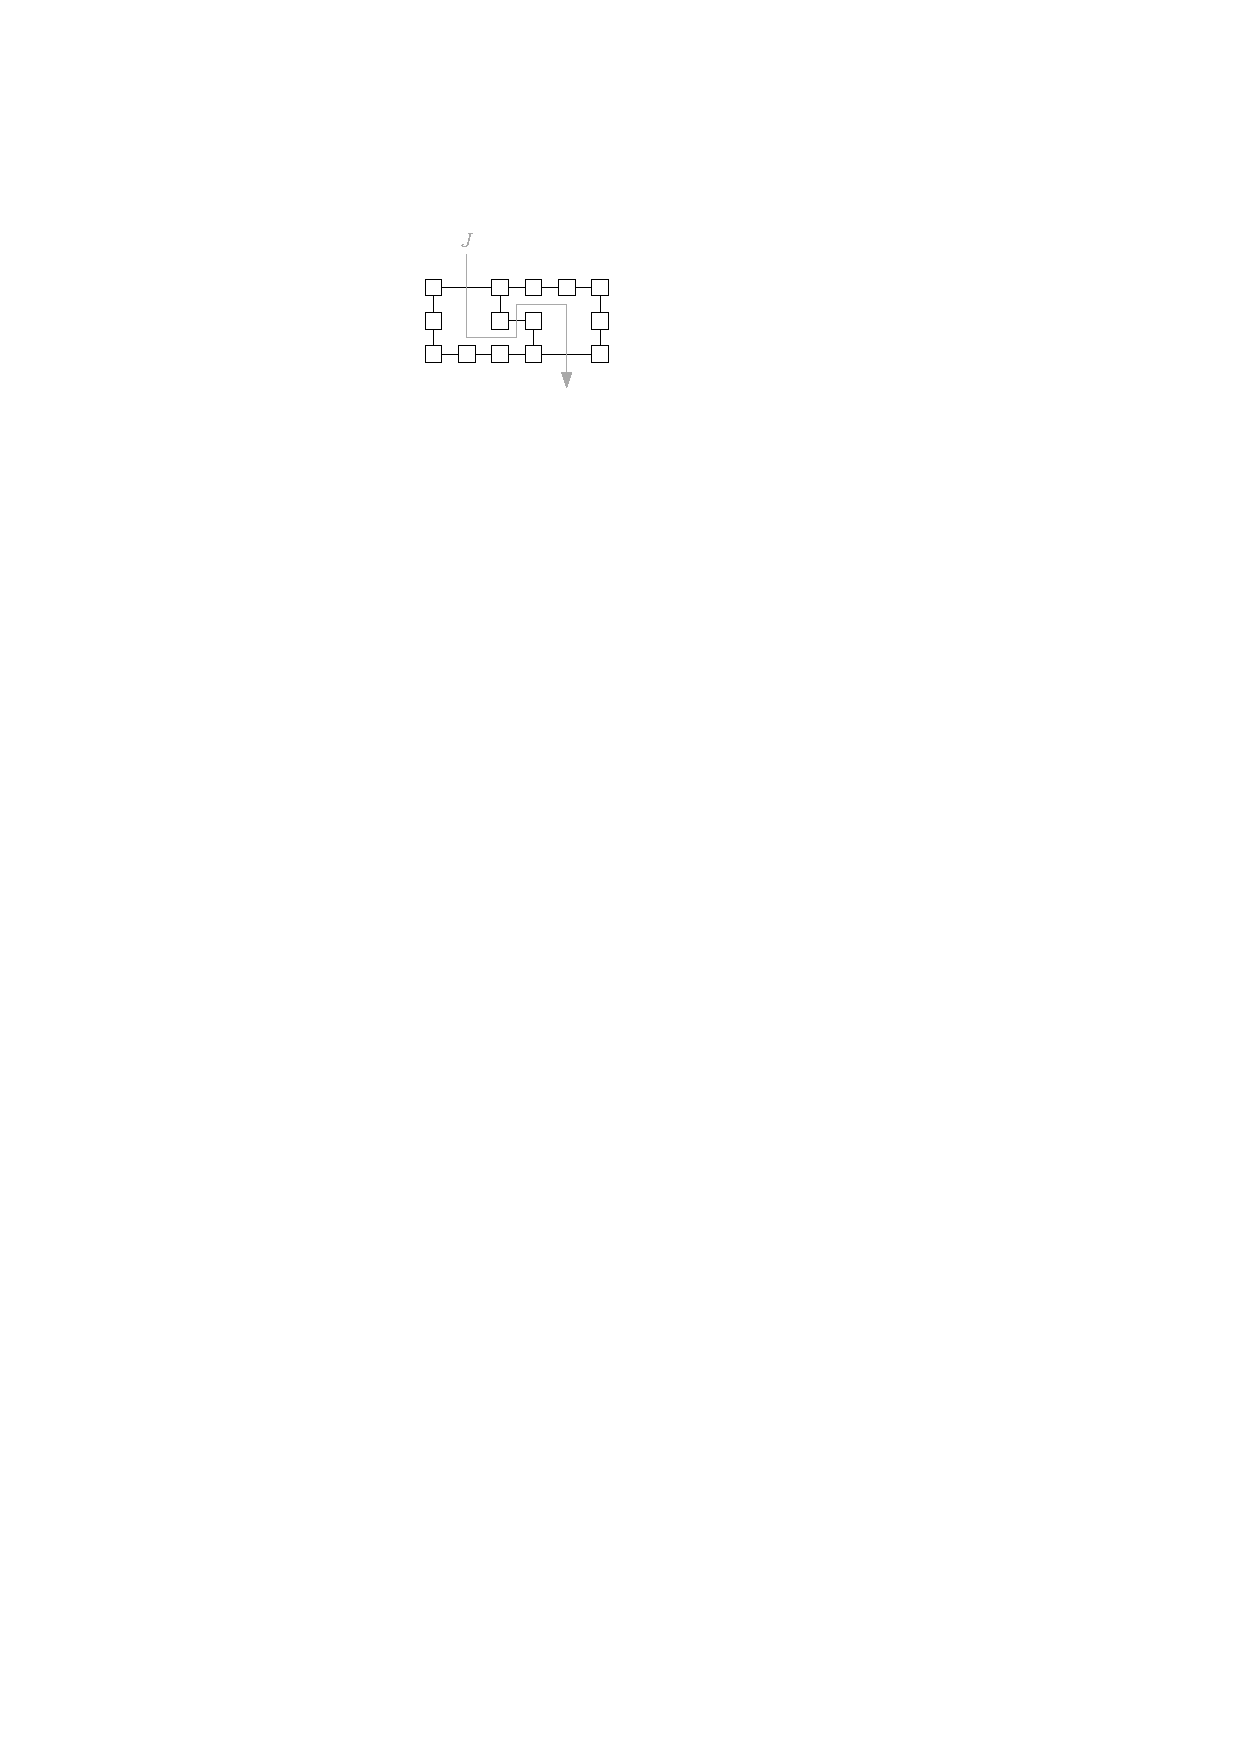
\includegraphics[width=0.6\linewidth,page=1]{includegraphics/4M_Moving_example.pdf}
		\caption{Illustration of the moving line $J$}
	\end{subfigure}
\begin{subfigure}{0.4\textwidth}
	\centering
	\includegraphics[width=0.48\linewidth,page=2]{includegraphics/4M_Moving_example.pdf}
	\caption{After the moving operation}
\end{subfigure}
\caption{With help of the moving line, four units are saved horizontally in total}\label{4M_ex2}
\end{figure}
In Figure \ref{4M_ex2}, an example is given for $J$ crossing a drawing simultaneously upwards and downwards. Notice, that the number of bends is preserved with the moving operation. The reason lies in the fact that the horizontal line segments, which are crossed by $J$, have the length of at least two.
%\subsubsection*{Matching}
%This operation is designed to save bends in a drawing. If there is a bend $b$ on a polyedge $e = (u,v)$, this method tries to move either $u$ or $v$ to $b$ in order to match a bend with a vertex. The matching operation is very similar to the moving operation. One difference is, that the so-called \textit{matching line} $J$ does not have to cross a border edge of the drawing, so the matching does not save area.
%\begin{definition}[Matching line $J$]
%	A bend-saving matching line $J$ is a line that fulfills the following conditions (let $s$ be the segment of $e$ between $v$ and $b$):
%	\begin{itemize}
%		\item $J$ is directed and consists of horizontal and vertical line segments
%		\item $J$ starts and ends in the face at the side of $e$ where $b$ has its 270\degree-angle and intersects the segment $s$
%		\item $J$ does not intersect any vertical edge of $\Gamma''$
%		\item Every horizontal edge of $\Gamma''$ besides $s$ that is intersected by a piece of $J$ which is directed downward has a finite length larger than the length of $s$
%	\end{itemize}	
%\end{definition}
%\begin{figure}[H]
%	\centering
%	\begin{subfigure}{0.4\textwidth}
%		\centering
%		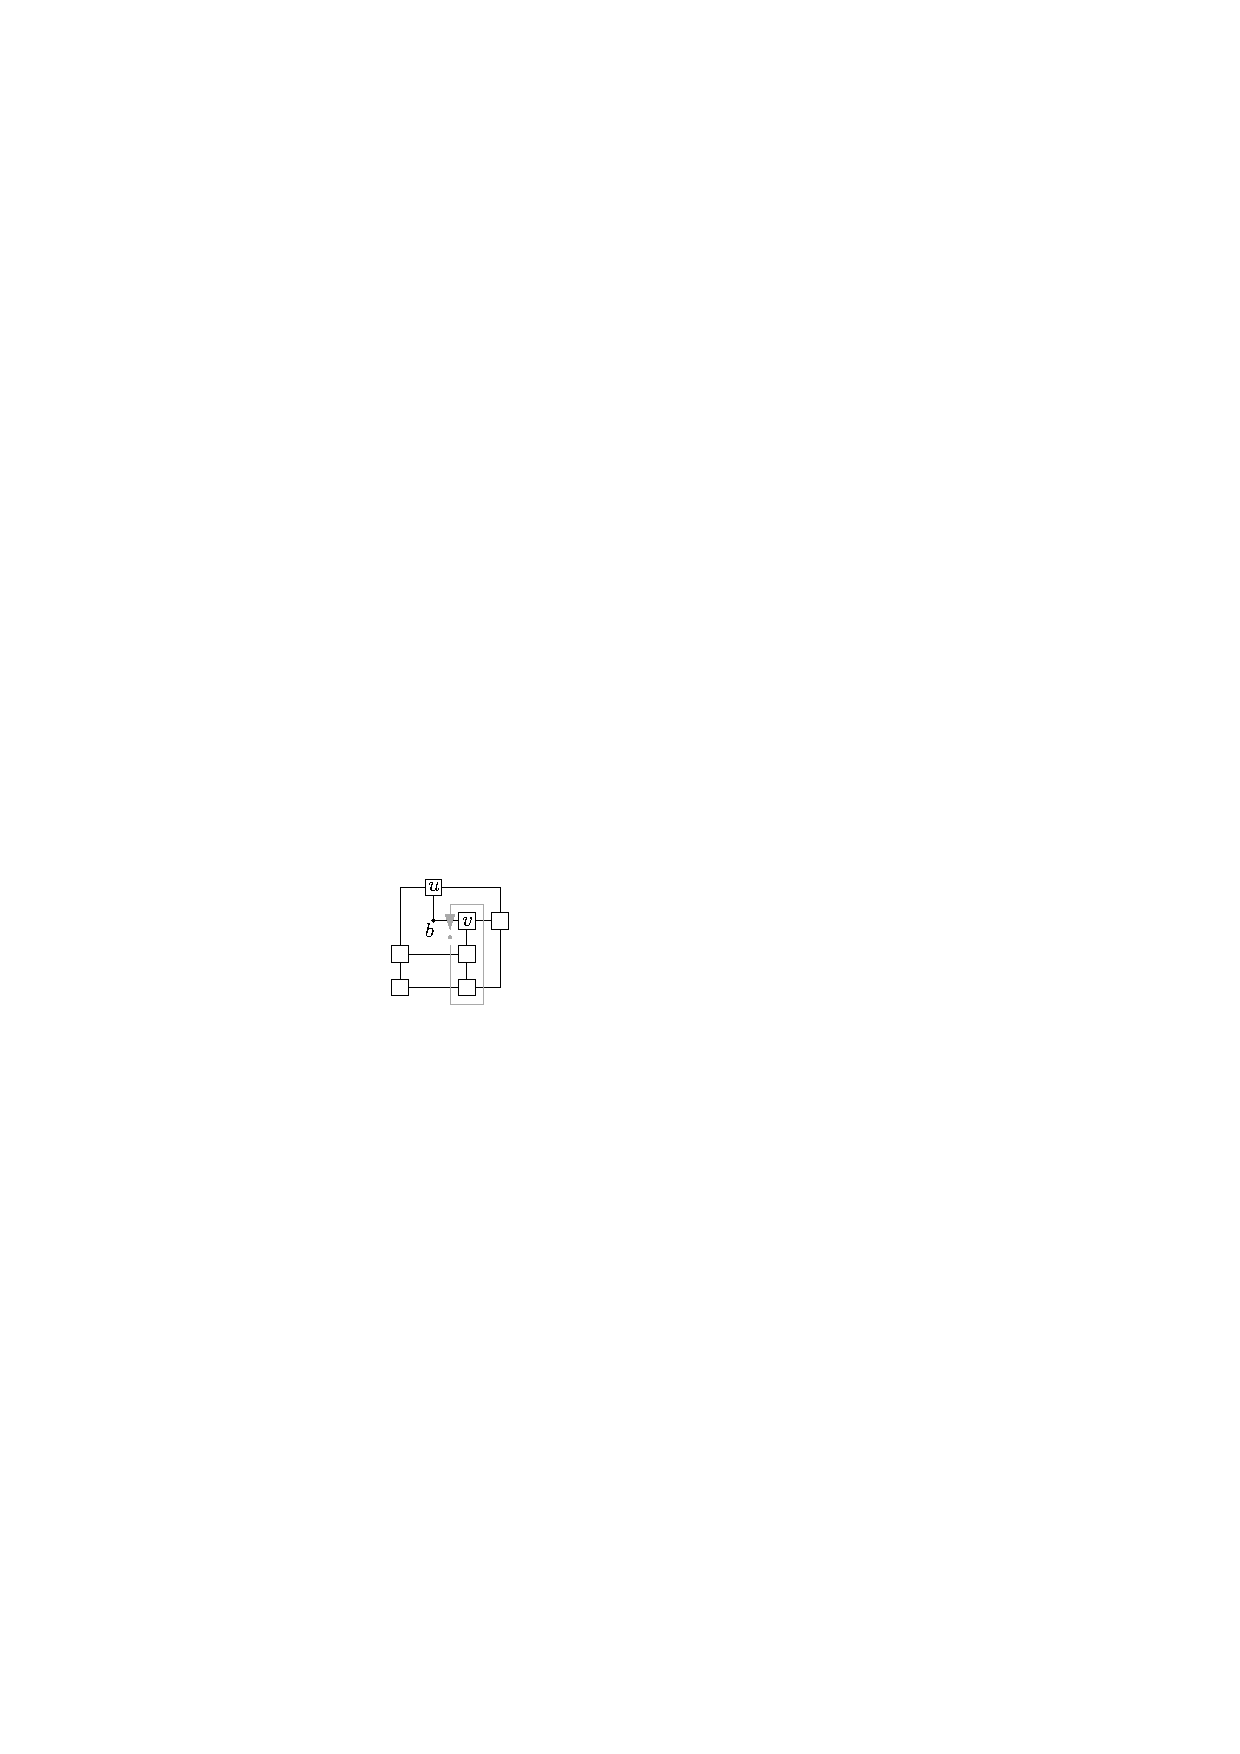
\includegraphics[width=0.6\linewidth,page=1]{includegraphics/4M_Matching_example.pdf}
%		\caption{Illustration of the moving line $J$}
%	\end{subfigure}
%	\begin{subfigure}{0.4\textwidth}
%		\centering
%		\includegraphics[width=0.6\linewidth,page=2]{includegraphics/4M_Matching_example.pdf}
%		\caption{After the moving operation}
%	\end{subfigure}
%	\caption{With help of the matching line, one bend is saved in total}
%\end{figure}
\subsection{Topology Shape Metrics}\label{def:topology_shape_metrics}
The process from a graph as a mathematical tuple to a drawing requires an appropriate embedding in order to guarantee special properties such as planarity or a statement regarding the number of bends. Tamassia et al. presented an algorithm resulting in orthogonal drawings with a minimal number of bends for a given embedding. Surprisingly, computing the minimal number of bends of an orthogonal graph embedding is in $P$. The whole process is called \textit{Topology Shape Metrics} \cite{Tamassia}. This procedure is rather flexible in its applications as we will see onwardly.\\
The computation of an orthogonal drawing with a minimal number of bends of a simple graph basically divided into three phases - the \textit{Topology phase}, the \textit{Shape phase} and the \textit{Metrics phase}.
\begin{itemize}
	\item \textit{Topology phase}\\
	This phase is initially used when there is no embedding specified in the first place. In this phase, a planar embedding on the plane is computed for the given graph.
	\item \textit{Shape phase}\\
	This phase is also called the \textit{orthogonalization phase}. The bends and its respective degrees of all the edges are computed along with the angles between the edges around a vertex. The result is an orthogonal representation.
	\item \textit{Metrics phase}\\
	Also known as the \textit{compaction phase}. Finally, the length of the edges and the position of the vertices are computed. The goal is to minimize the area the graph demands.
\end{itemize}
Every phase can be adjusted for special needs. As already mentioned, the Topology Shape Metrics approach serves as a standard practice in research due to its flexibility.\cite{podevsaef}

\subsection{Previous results}
Our main goal is to smoothen the orthogonal drawings by introducing circular arcs. We will consider quarter and semi circular arcs in order to achieve a smoothened 90\degree~bend.
\begin{definition}[Smooth Orthogonal Layout - \textit{SMOG} in short, {\cite{SMOG}}]
	A \textit{Smooth Orthogonal Layout} of a 4-planar graph $G$ is a graph where
	\begin{itemize}
		\item each vertex of $G$ is drawn as a point on the plane;
		\item each edge of $G$ is drawn as a sequence of axis aligned line segments and circular arc segments. The segments have to intersect in a point. The tangent at this point has to be horizontal or vertical, just as the segments itself;
		\item planarity is preserved;
		\item a port of a vertex is incident to at most one edge.
	\end{itemize}
\end{definition}
A smooth orthogonal layout inherits a so-called \textit{edge complexity} $k \geq 1$, if there does not exist any edge with complexity $k+1$ or greater. The smooth orthogonal layout derives from an orthogonal drawing by postprocessing algorithms. The positions of vertices are altered in the horizontal direction.
In fact, the smooth orthogonal layout representation of 4-planar graphs are already intensively studied regarding area bounds, complexity increase and the number of bends. Recall that the vertices of a 4-planar graph can have at most one edge per port - one each for North, South, West, East - and are illustrated as a point in the plane.
\subsubsection{Fixed Layout Model}
Considering an orthogonal drawing of a graph $\Gamma_G$ in the Fixed Layout Model, the position of the vertices cannot be altered. This is a rather strict constraint. The implementation of circular arcs in a polyline lead to an increase of the edge complexity. Every bend is substituted with a quarter arc, resulting in two new bends in the worst case.
\begin{theorem}[{\cite[p. 581, Figure \ref{im:4-staircase}]{SMOG}}]
	In the Fixed Layout Model, the edge complexity of a given orthogonal graph $G$ might increase from $k$ to $2k-1$.
\end{theorem}
\begin{figure}[H]
	\centering
	\begin{subfigure}{.4\textwidth}
    \centering
	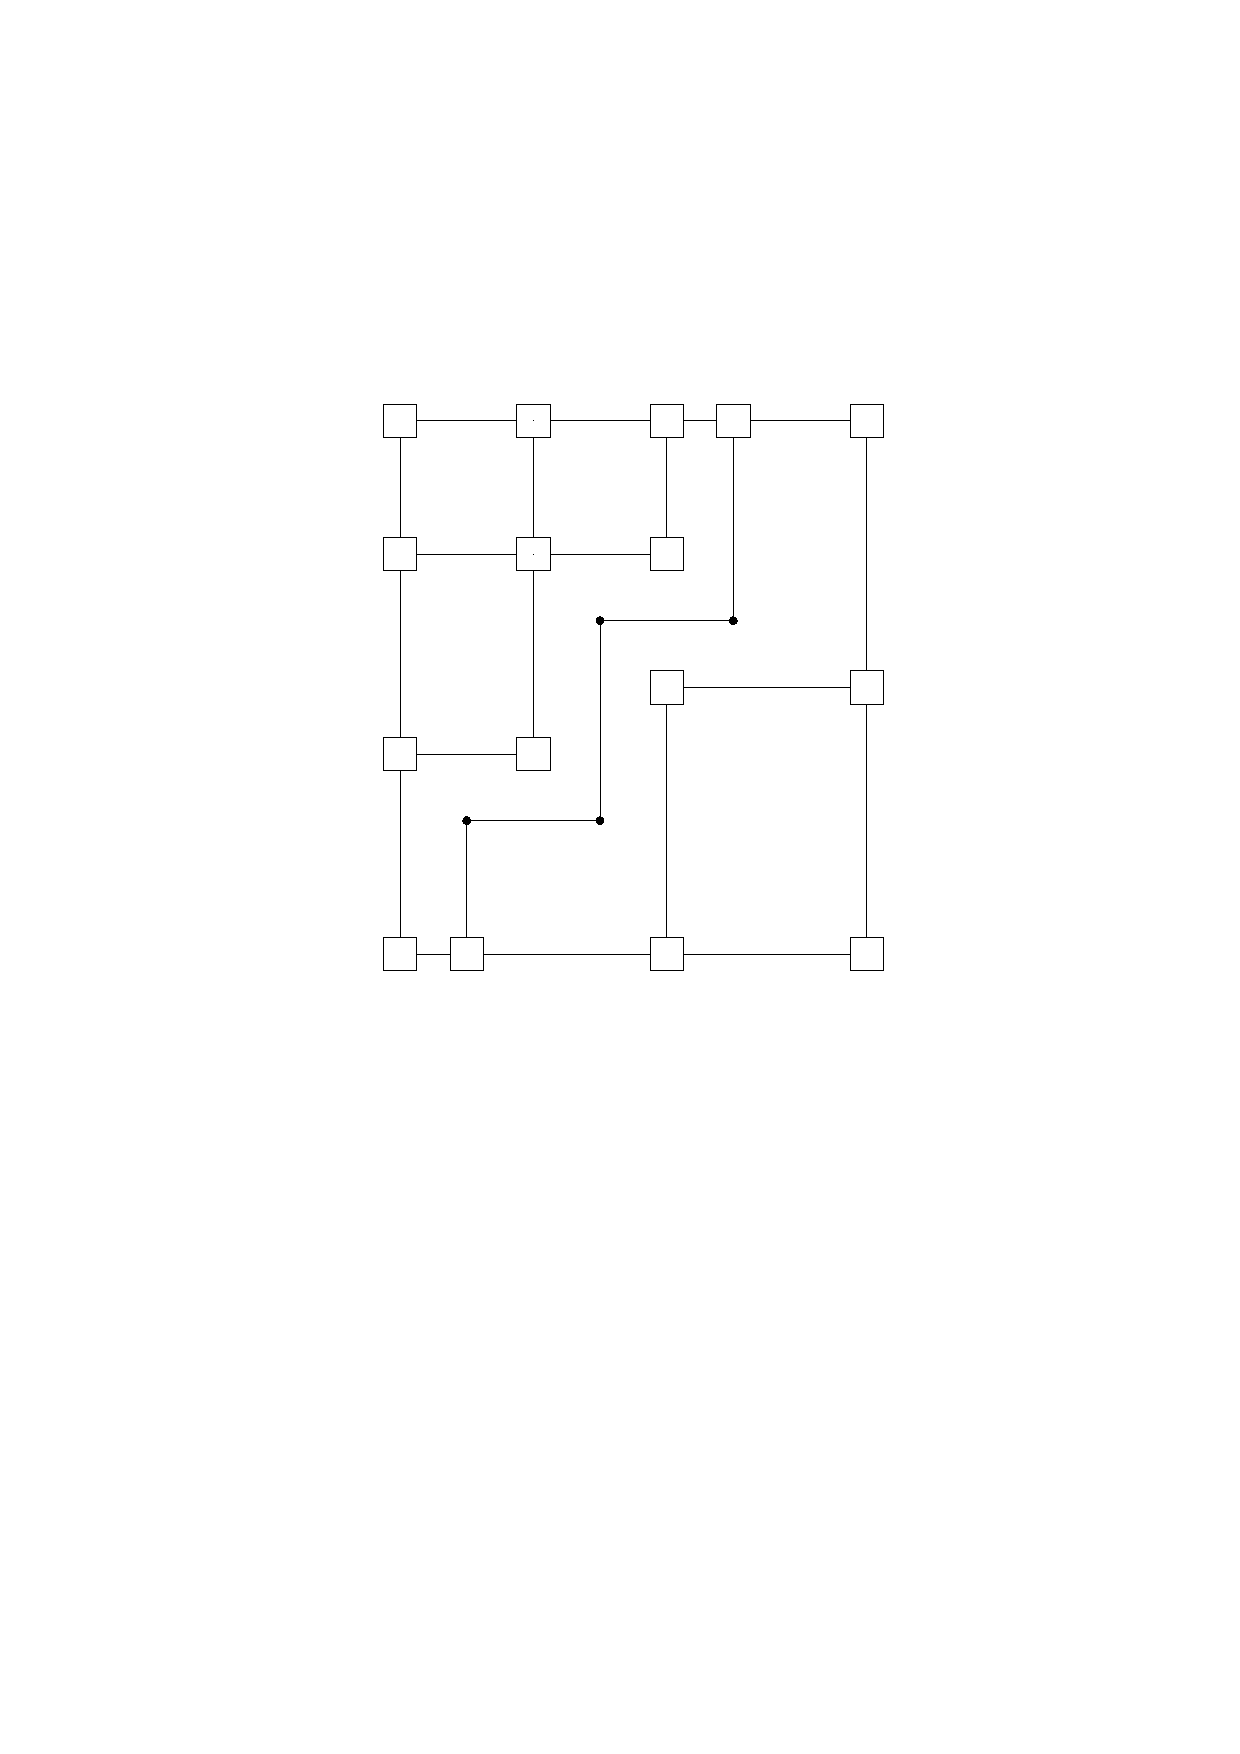
\includegraphics[width=0.7\linewidth,page=1]{includegraphics/staircase-4-planar.pdf}
	\caption{Staircase in Kandinsky}	
	\end{subfigure}
\begin{subfigure}{.4\textwidth}
	\centering
	\includegraphics[width=0.7\linewidth,page=2]{includegraphics/staircase-4-planar.pdf}
	\caption{SMOG representation}
\end{subfigure}
\caption{The complexity increase of 4-planar graphs with staircases}\label{im:4-staircase}
\end{figure}
The reason for the edge complexity increase is the fixation of the vertices and following example regarding so-called \grqq Staircase Edges\grqq.
Regarding the significant rise of complexity and due to the fact, that circular arcs with a very small radius might be introduced, the Fixed Layout Model might not be suitable for smoothening an orthogonal drawing. Circular arcs with a small radius might not emphasize the ongoing direction of the edge, therefore for the viewers eye. A different approach is the Fixed Shape Model, where the orthogonal representation is preserved (the circular ordering of the polyedges around a vertex).
\subsubsection{Fixed Shape Model}
In the Fixed Shape Model, the circular ordering of the edges connected to a vertex is preserved. The vertices are of uniform size but can be repositioned on the coarse integer grid. 
\begin{definition}[Stretching technique, {\cite[p. 582]{SMOG}}]
	The stretching technique is a process where every horizontal edge of a given orthogonal drawing is elongated by the length of the longest vertical segment $l$ of the drawing. The result is an orthogonal drawing of size up to $\Rho(n^2) \times \Rho(n)$, where $n$ is the number of vertices.
\end{definition}
Due to the horizontal stretching technique by the factor of $l$, there is new space left and right from every vertical line segment. To be more precise, there is an empty box left and right from every vertical line with size $l'\times l'$, while $l'$ is the length of the respective vertical line.\cite[p. 583, Figure 5]{SMOG}\\
In practice, the SMOG Model is derived from the Kandinsky Model using basically two plane sweeps: The first plane sweep stretches the Kandinsky drawing horizontally by the factor of the longest vertical line segment. This plane sweep holds horizontal line segments as events. Every time a new horizontal line segment gets active, all the active segments are extended by $l$. This results in a stretching of every grid cell. The second plane sweep substitutes parts of the horizontal and vertical line segments with corresponding quarter circular arcs, making the drawing \textit{smooth}. The resulting drawing is in $\Rho(n^2) \times \Rho(n)$ area due to the horizontal stretching.
The worst case of the stretching technique results in a quadratic size of width. Consider the following example:
\begin{figure}[H]
	\centering
	\begin{subfigure}{.4\textwidth}
		\centering
		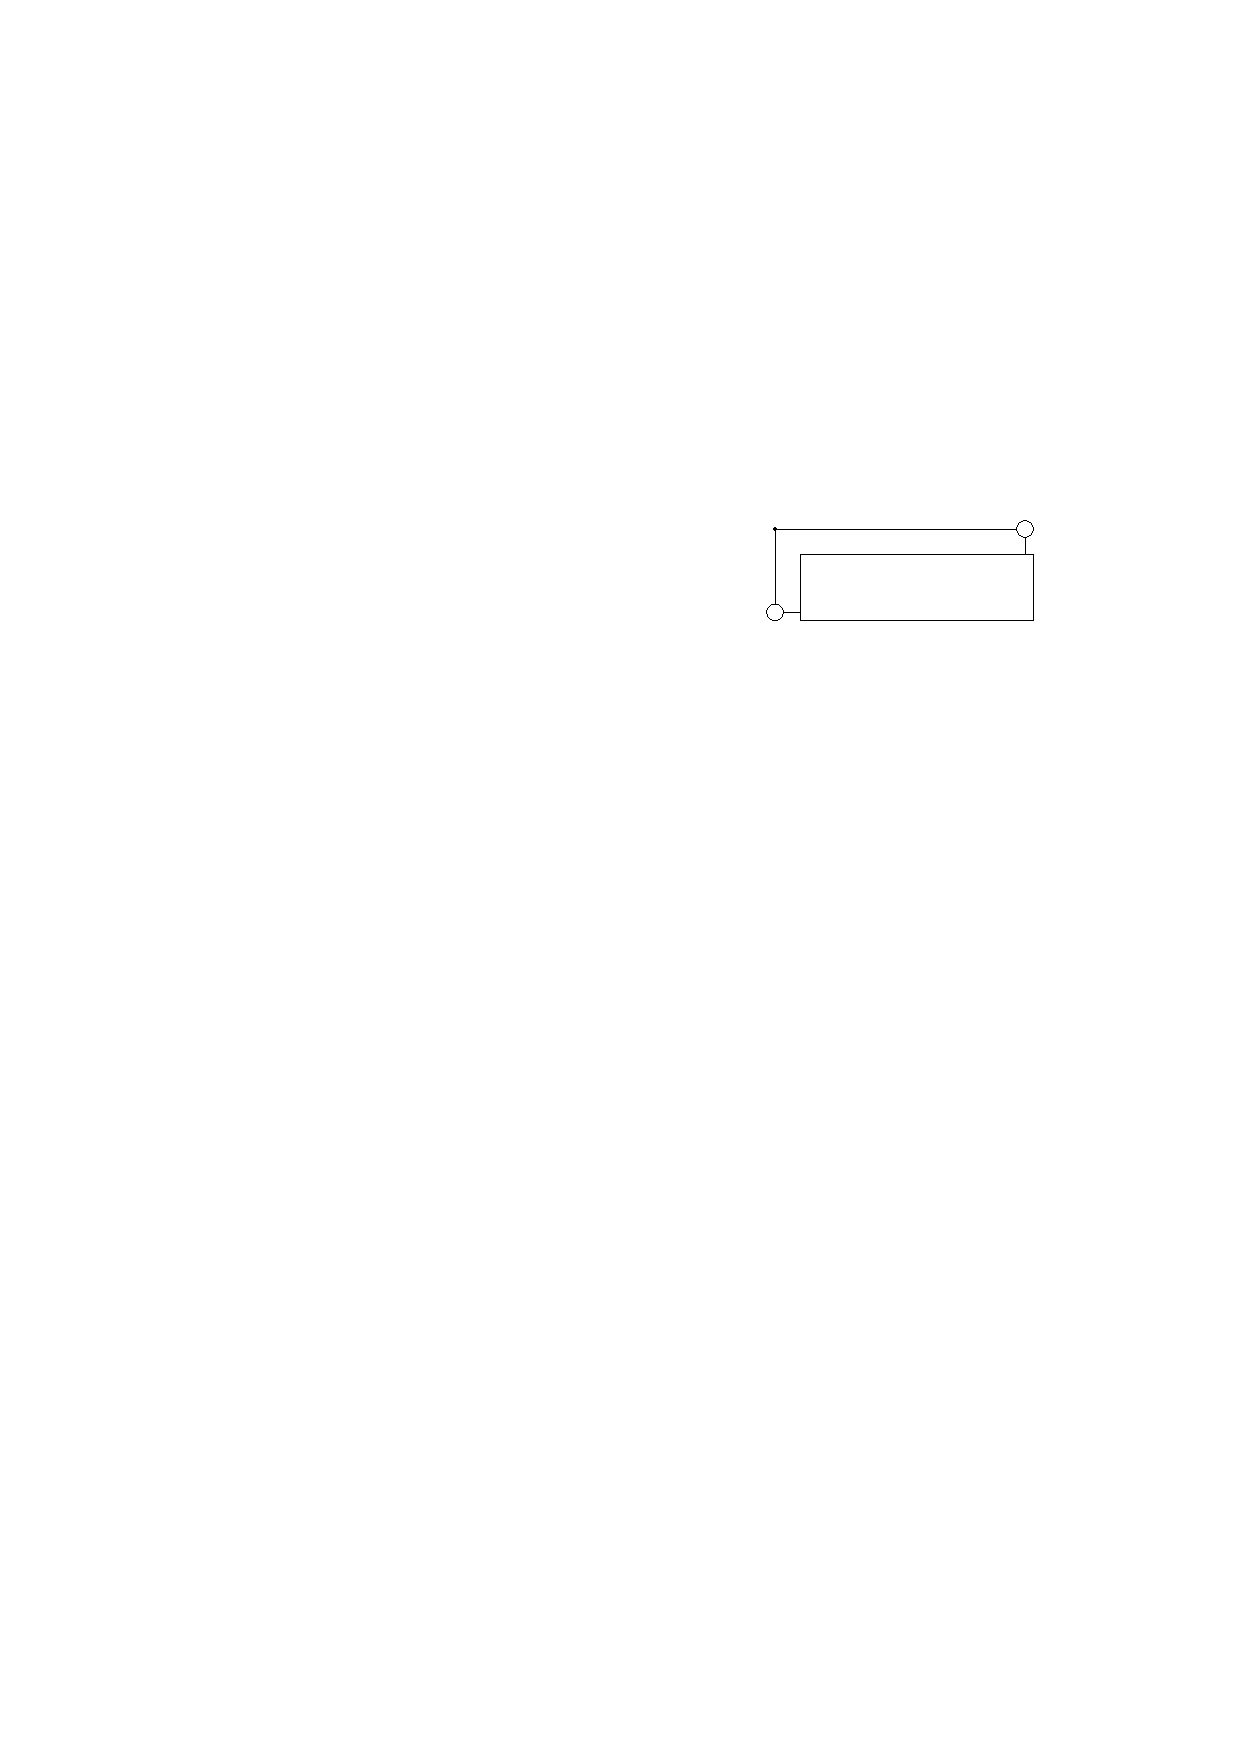
\includegraphics[width=0.7\linewidth,page=1]{includegraphics/4-planar_worst_case.pdf}
		\caption{Original orthogonal graph}	
	\end{subfigure}
	\begin{subfigure}{.6\textwidth}
		\centering
		\includegraphics[width=0.9\linewidth,page=2]{includegraphics/4-planar_worst_case.pdf}
		\caption{After applying the stretching technique}
	\end{subfigure}
	\caption{Worst case illustration of the stretching technique}\label{im:4-planar_worst_case}
\end{figure}
The box in Figure \ref{im:4-planar_worst_case} illustrates a grid of vertices which is of size $\Rho(n)\times\Rho(n)$. There are therefore $\Rho(n)$ edges in the box horizontally and the polyedge of the outermost vertices contains a vertical segment of size $\Rho(n)$. By applying the stretching technique, the horizontal segment of the outer polyedge gets $\Rho(n)$ additions in length of size $\Rho(n)$, resulting in $\Rho(n^2)\times\Rho(n)$ area.
\begin{theorem}[{\cite[p. 584]{SMOG}}]
	If the bends of a polyline are purely \underline{uniform} (in the same direction), then there is a SMOG representation of that polyline without an increase of complexity. Similarily, if the polyline is purely \underline{alternating}, the edge complexity raises from $k$ to $\lceil\frac{3}{2}k\rceil$.
\end{theorem}
\begin{sketch}
	If a polyline is purely uniform, consider the vertical segments as follows; If a vertical segment lies between two horizonal segments, substitute that vertical segment with a semicircle arc. If a vertical segment is connected to a vertex and a segment, substitute the vertical segment with a quadrant arc. If the polyedge consists of one vertical segment, then two vertices are at both ends. The edge complexity is not altered (Figure \ref{im:4-uniform}). The space around a vertical segment, necessary for the circle arc substitution, is guaranteed by stretching the entire drawing horizontally by a factor of the longest vertical segment.\\
\begin{figure}[H]
\centering
\begin{subfigure}{0.4\linewidth}
	\centering
	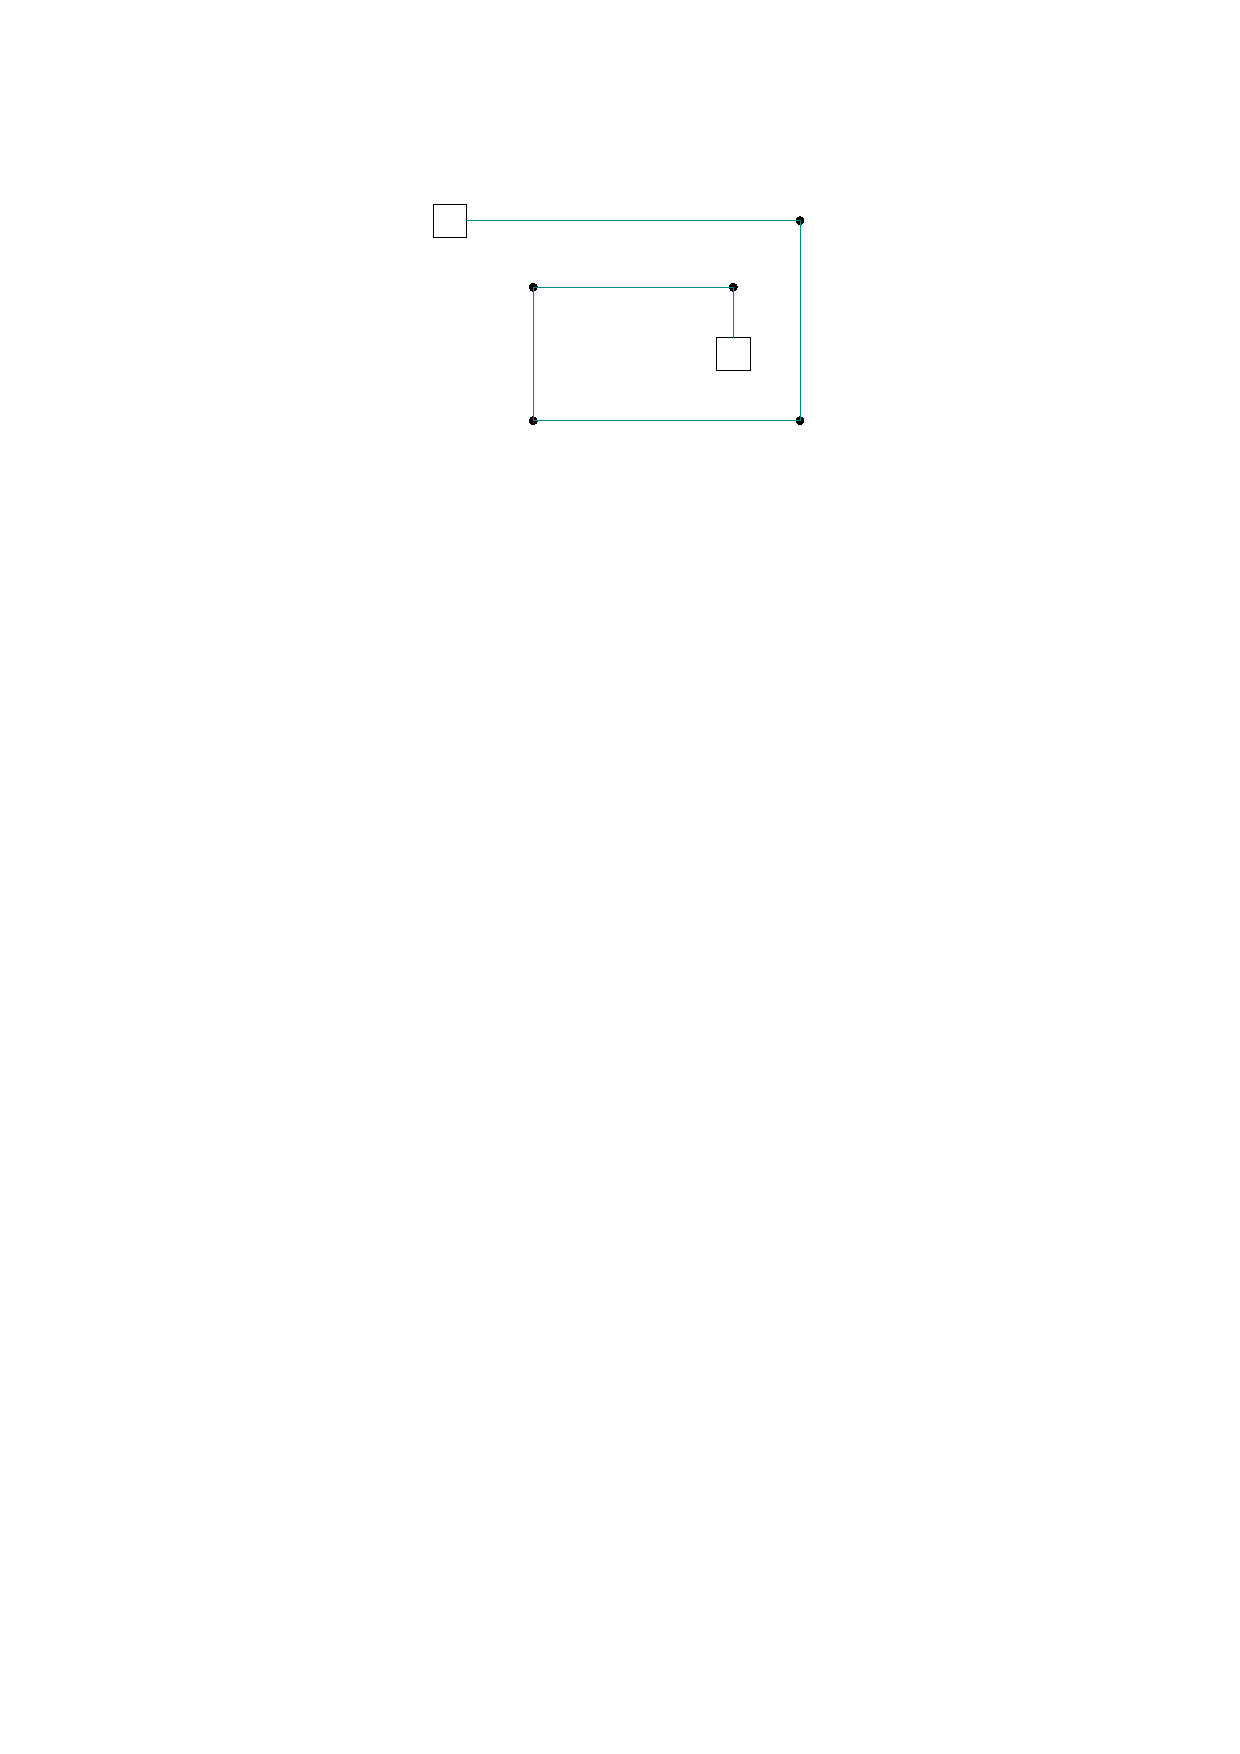
\includegraphics[width=0.5\textwidth,page=1]{includegraphics/smogify_uniform_staircase.pdf}
	\caption{Uniform polyedge with 5 bends}
\end{subfigure}
\begin{subfigure}{0.4\linewidth}
	\centering
	\includegraphics[width=0.9\textwidth,page=2]{includegraphics/smogify_uniform_staircase.pdf}
	\caption{No complexity increase in SMOG}
\end{subfigure}
\caption{The uniform case - No complexity increase under $\Rho(n^2)\times\Rho(n)$ area}\label{im:4-uniform}
\end{figure}
Similarily, if the polyline is purely alternating, then due to the stretching technique the area of $|l'|\times |l'|$ left and right of a vertical segment $l'$ is still guaranteed. We are able to substitute the staircase with same sized circular arcs with alternating turns, increasing the total number of bends from $k-1$ to $\lfloor\frac{3}{2}k\rfloor$ (Figure \ref{im:4-alter}).\\
\begin{figure}[H]
\centering
\begin{subfigure}{0.45\linewidth}
	\centering
	\includegraphics[width=0.35\textwidth,page=3]{includegraphics/smogify_uniform_staircase.pdf}
	\caption{Alternating polyedge with 5 bends}
\end{subfigure}
\begin{subfigure}{0.4\linewidth}
	\centering
	\includegraphics[width=1\textwidth,page=4]{includegraphics/smogify_uniform_staircase.pdf}
	\caption{Complexity increase in SMOG}
\end{subfigure}
\caption{The alternating case - Complexity increase under $\Rho(n^2)\times\Rho(n)$ area}\label{im:4-alter}
\end{figure}
\end{sketch}
\begin{theorem}
	Let $G$ be a 4-planar graph with an orthogonal drawing $\Gamma_G$. If any polyline is alternating at some point, it is possible that $\Gamma_G$ can be minimized regarding the number of bends. \label{th:alt_not_min}
\end{theorem}
\begin{sketch}
	We show the theorem by flow minimization over the dual graph the following way: Let $e$ be a polyedge seperating two faces $f,g$. For each convex bend in the face $f$, we send one unit of flow from $f$ to $g$ and vice versa. If there is an alternation in $e$, then there is a cycle of flow between $f$ and $g$ and the edge can be minimized.%the unit of the minimized flow and the direction between both faces determines the minimal direction changes of an edge resulting in a lower number of bends.
\end{sketch}
The flow minimization is an application of Tamassia \cite{Tamassia}. It is possible that this minimization actively changes the shape in some point, arising a new model - the \grqq Almost Fixed Shape\grqq~model \cite{LombardiFlow}.
\begin{theorem}
	In the Fixed Shape Model, an orthogonal graph $G$ - with minimal number of bends and an edge complexity of $k$ - can be transferred to a SMOG without an edge complexity increase under $\Rho(n^2) \times \Rho(n)$ area.
\end{theorem}
\begin{sketch}
	If $G$ has got a minimal number of bends, then there is no alternation in any polyline by contraposition of Theorem \ref{th:alt_not_min}. The polyedges are purely uniform and every vertical segment is replaced by either a quarter circle arc or a semicircle arc or it stays the same. As we already saw, uniform bends do not lead to an edge complexity increase. Planarity is preserved due to the stretching technique.
\end{sketch}
\subsection{Drawings with low complexity}
The persistance of some bends lies in the orthogonality property of the drawing. If two vertices connected by a polyedge do not share the same $x$ or $y$ coordinate, then the polyedge has to overcome the differences in the regarding direction with horizontal and vertical segments, preserving the port constraint.
\begin{figure}[H]
	\centering
	\begin{subfigure}{0.6\linewidth}
		\centering
		1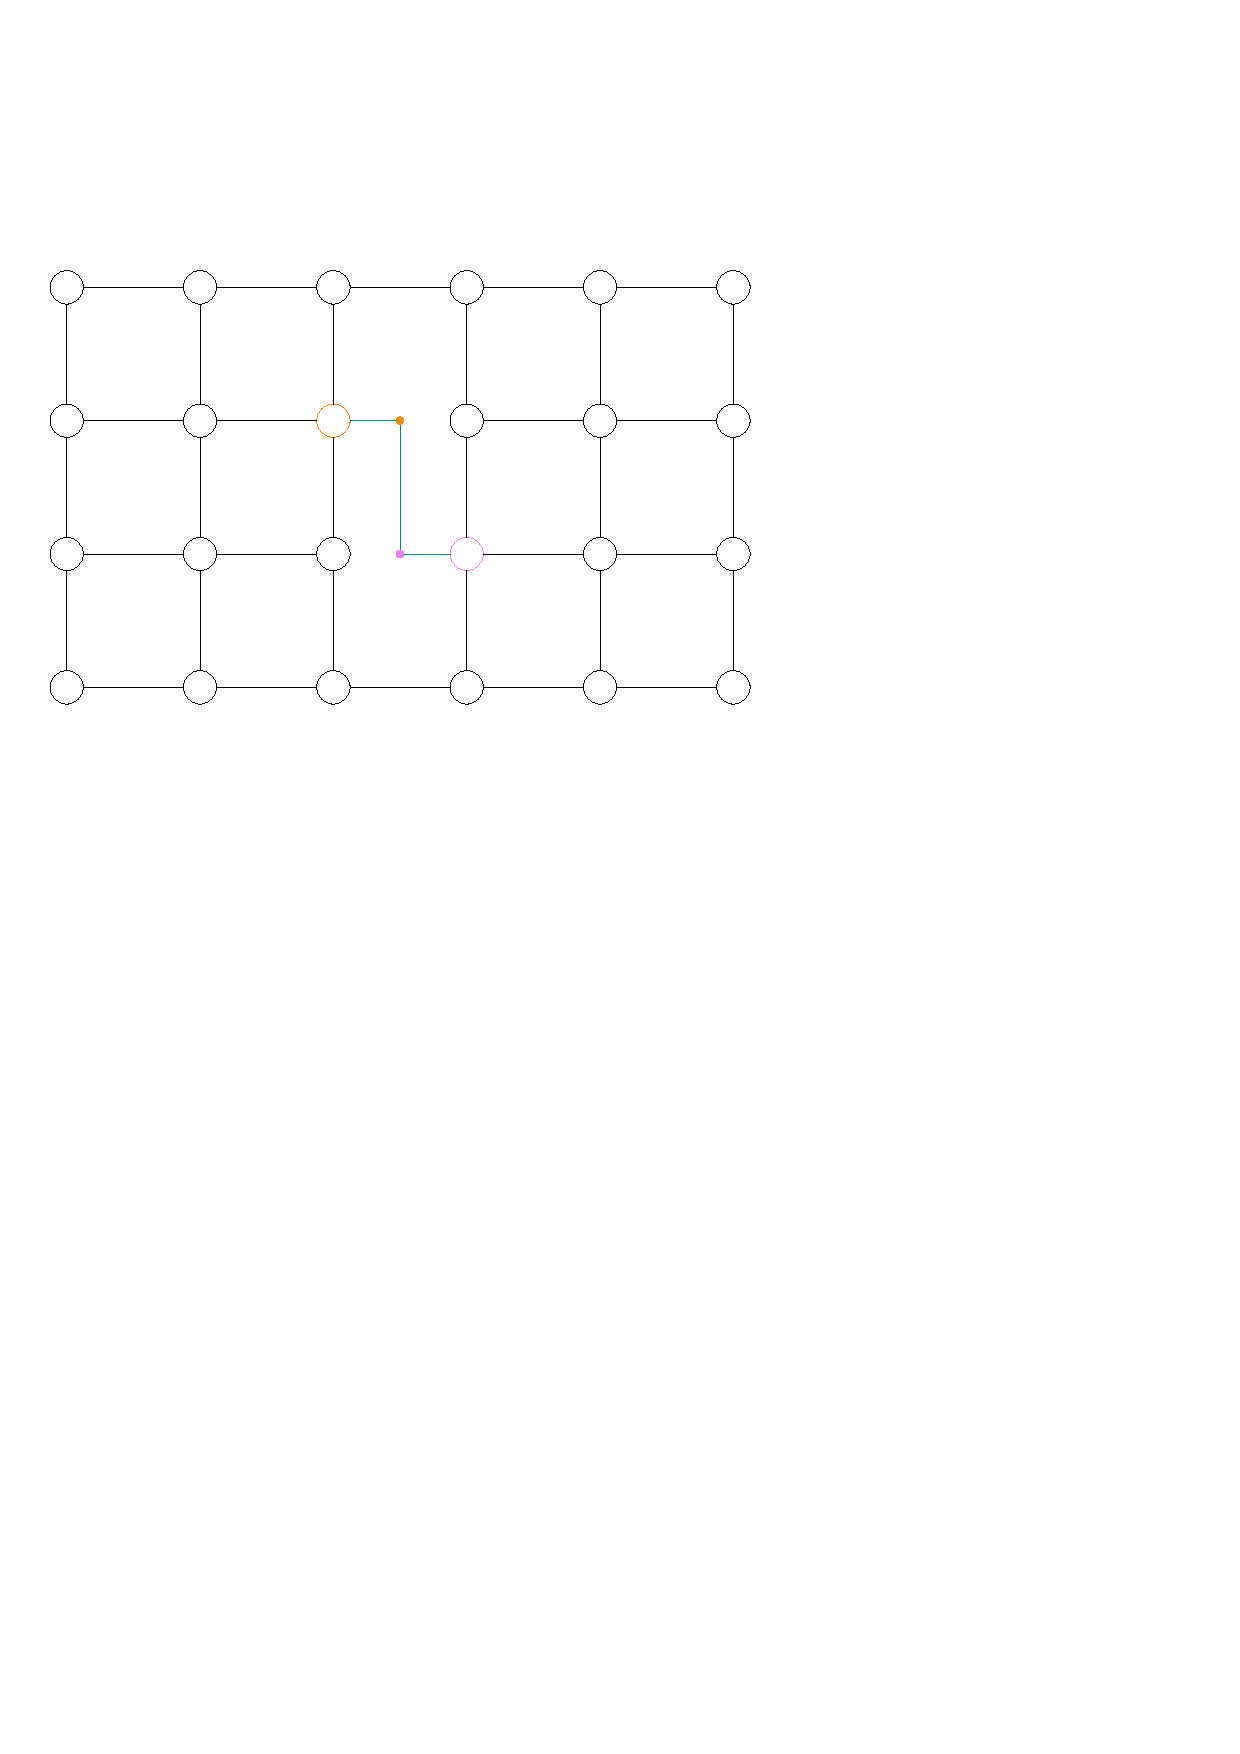
\includegraphics[width=0.7\textwidth,page=1]{includegraphics/kandinsky_bends.pdf}
	\end{subfigure}
	\caption{A drawing with a staircase of complexity 3}\label{im:kandinsky_bends}
\end{figure} 
In Figure \ref{im:kandinsky_bends}, we see an orthogonal drawing of a 4-planar graph a staircase edge of complexity 3. Notice that the cyan coloured polyedge is zig-zag shaped.
\begin{theorem}[{\cite[Theorem 3, p. 583]{SMOG}}]
	Let $G$ be a 4-planar graph with an orthogonal drawing $\Gamma_G$ of complexity 3. Then, there is a complexity-4 smooth orthogonal layout in $\Rho(n^2) \times \Rho(n)$ area.\label{th:3to4}
\end{theorem}
\begin{sketch}
	By the stretching technique, the space for arc substitution is guaranteed. For complexity-1 or complexity-2 edges, the complexity does not increase. Alternating complexity-3 edges will increase from 3 to 4.
\end{sketch}
\begin{figure}[h]
	\centering
	\begin{subfigure}{0.6\linewidth}
		\centering
		\includegraphics[width=0.7\textwidth,page=2]{includegraphics/kandinsky_bends.pdf}
	\end{subfigure}
	\caption{Smooth orthogonal layout of figure \ref{im:kandinsky_bends}}\label{im:kandinsky_bends2}
\end{figure} 
In Figure \ref{im:kandinsky_bends2}, the drawing of figure \ref{im:kandinsky_bends} got stretched and circular arcs were substituted, resulting in a complexity-4 smooth orthogonal layout.
\subsection{\NP-hardness}
It is proved by Bekos et al. that it was \NP-hard to decide whether a 4-planar graph with a given representation admits a bendless SMOG. To be more precise:
\begin{theorem}
	Given a planar graph $G$ of max-degree 4 and a SMOG representation $\mathcal{R}$, it is \NP-hard to decide whether $G$ admits a bendless SMOG preserving $\mathcal{R}$. This is the implementation of the last step of the Topology Shape Metrics approach (Bend minimization by Tamassia, in $P$ for orthogonal drawings). %The \NP-hardness still holds even if $\mathcal{R}$ requires all edges to be drawn as straight-line segments or quarter circular arcs.
	\label{th:NP-hard-4}
\end{theorem}
\begin{sketch}
	The proof inherits a reduction from 3-\call{SAT} to a SMOG representation construction which is bendless if and only if a formula $\varphi$ given in CNF is satisfiable. $\Gamma_\varphi$ is constructed with so-called \textit{auxiliary gadgets}, where the information flows along the faces encoded in their length. There are multiple gadgets, as shown below. The vertices are illustrated as circles.
	\begin{itemize}
		\item \textit{Variable gadget}\\
		For each variable $x$ of $\varphi$, a variable gadget gets three edges of the same length $3\cdot l(u)$ as input. The assignment is encoded in the following way:
		\begin{align}
		x &= \texttt{True}  & &\Leftrightarrow  & l(x) &= 2\cdot l(u), l(\overline{x}) = 1\cdot l(u)\\
		x &= \texttt{False} & &\Leftrightarrow & l(x) &= 1\cdot l(u), l(\overline{x}) = 2\cdot l(u)
		\end{align}
		\begin{figure}[H]
			\centering
			\begin{subfigure}{0.4\textwidth}
				\centering
				\includegraphics*[width=0.9\linewidth,page=1]{includegraphics/NP_4_variable_gadget.pdf}
				\caption{\texttt{true} assignment}
			\end{subfigure}
			\begin{subfigure}{0.4\textwidth}
				\centering
				\includegraphics*[width=0.9\linewidth,page=2]{includegraphics/NP_4_variable_gadget.pdf}
				\caption{\texttt{false} assignment}
			\end{subfigure}
			\caption{Variable gadgets for the 4-planar case}\label{im:4-variable-gadgets}
		\end{figure}
		\item \textit{Parity gadget}\\
		The parity gadget guarantees that a variable is defined as \texttt{true} or \texttt{false}. For instance, if $l(u) = 2$, then the variable gadget could set $l(x) = l(\overline{x}) = 3$ which is considered as an undefined variable.
		\begin{figure}[H]
			\centering
			\begin{subfigure}{0.4\textwidth}
				\centering
				\includegraphics*[width=0.9\linewidth,page=1]{includegraphics/NP_4_parity_gadget.pdf}
				\caption{\texttt{true} assignment}
			\end{subfigure}
			\begin{subfigure}{0.4\textwidth}
				\centering
				\includegraphics*[width=0.9\linewidth,page=2]{includegraphics/NP_4_parity_gadget.pdf}
				\caption{\texttt{false} assignment}\label{im:4-triangle}
			\end{subfigure}
			\caption{Parity gadget for the 4-planar case}\label{im:4-parity-gadgets}
		\end{figure}
	Consider the triangle illustrated in Figure \ref{im:4-triangle}. The center of the circular arcs shoujld be at distance greater than $2\cdot l(u)$. Consider $\lambda = l(\overline{x}) - l(x)$ as dependence, then the length of this segment can be expressed as follows: $\sqrt{4\lambda^2 + l(u)^2}$. So, to avoid crossings, $\lambda$ should value at least $\frac{\sqrt{3} }{2}\cdot l(u)$. It follows that $l(x),l(\overline{x} ) \in (0,1.067 l(u) )\cup (1.933 l(u),3)$ in order to avoid crossings.
		\item \textit{Clause gadget}\\ For each clause of $\varphi$ in CNF there is a gadget for the literals $a,b$ and $c$. The length composition guarantees that at least one of those literals must be \texttt{true}.
		\begin{figure}[H]
			\centering
			\begin{subfigure}{0.4\textwidth}
				\centering
				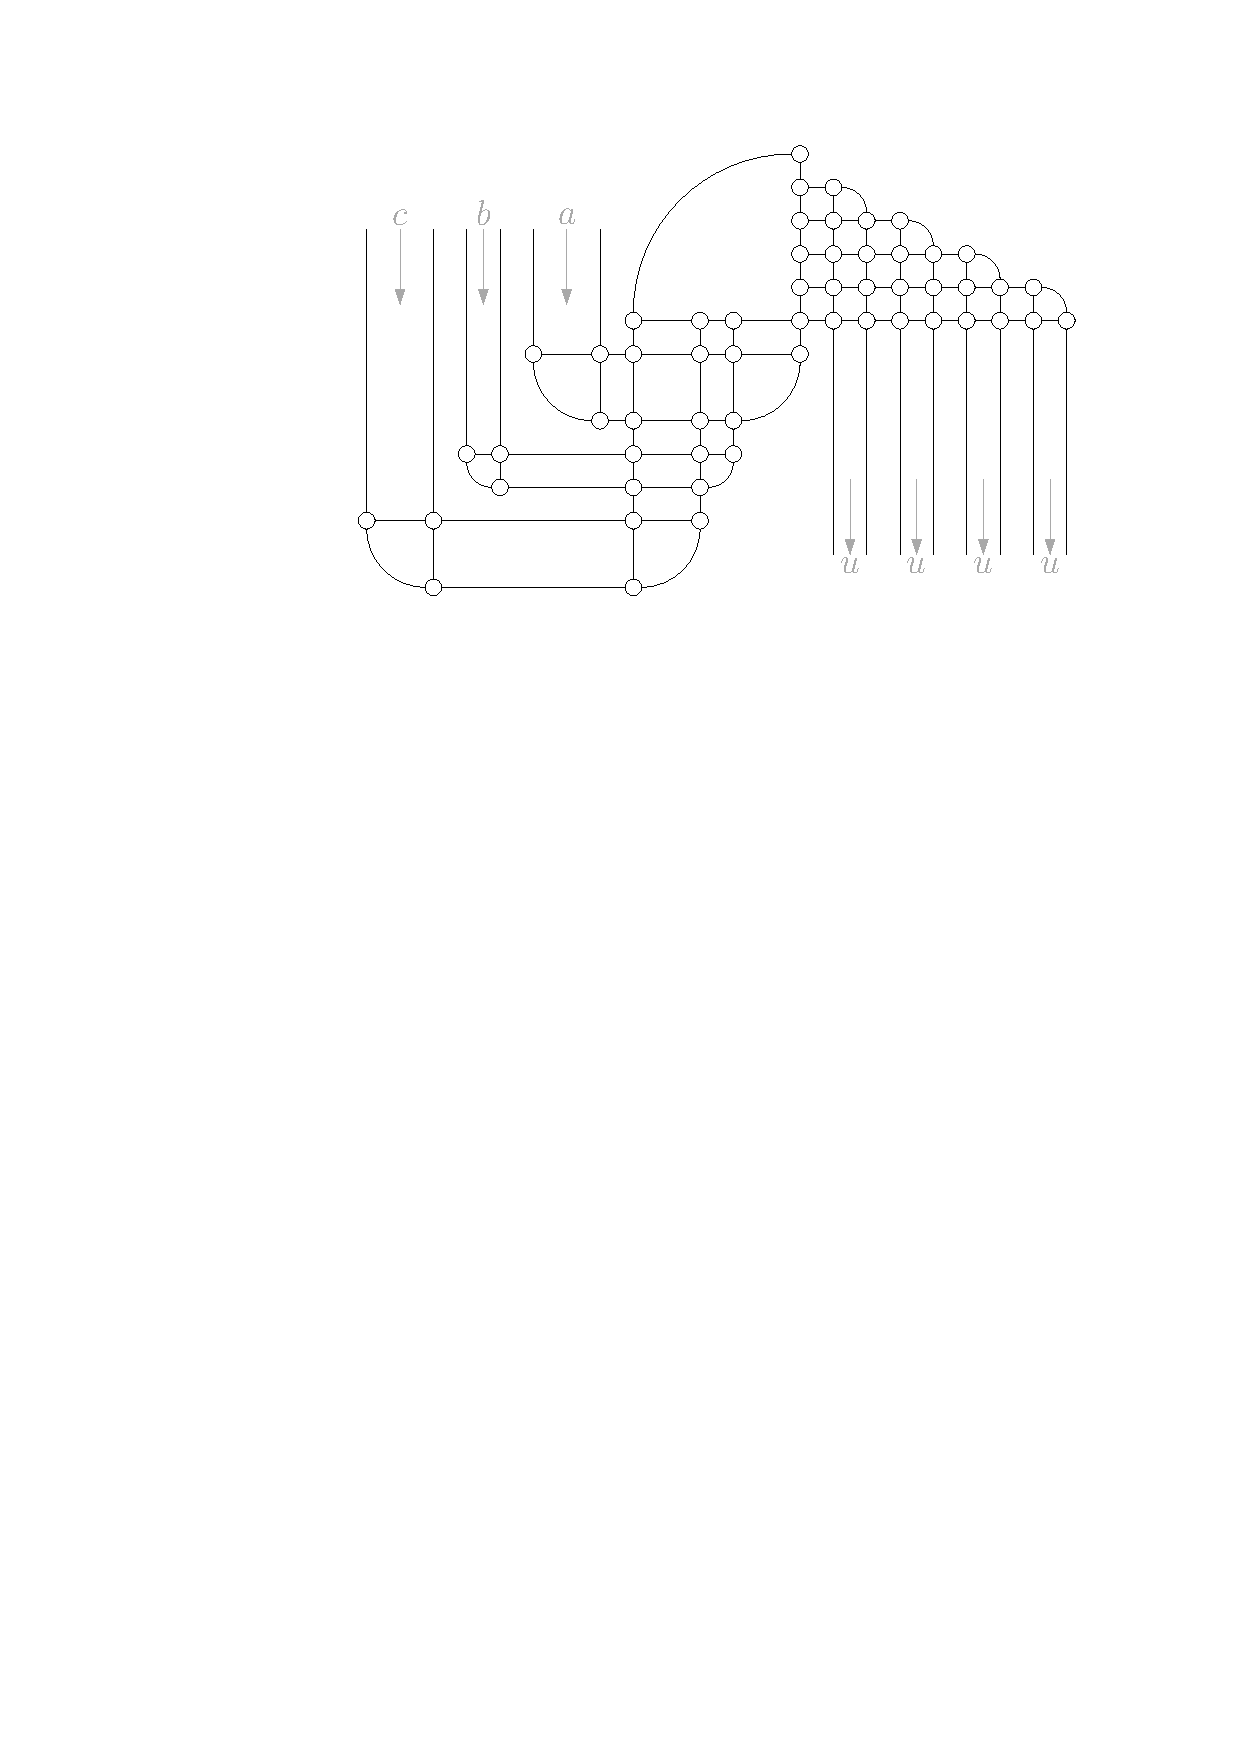
\includegraphics[width=0.9\linewidth,page=1]{includegraphics/NP_4_auxiliary_gadget.pdf}

			\end{subfigure}
						\caption{Clause gadget}
		\end{figure}
		\item \textit{Auxiliary gadget}\\
		\begin{figure}[H]
			\centering
			\begin{subfigure}{0.4\textwidth}
				\centering
				\includegraphics[width=0.4\linewidth,page=2]{includegraphics/NP_4_auxiliary_gadget.pdf}
				\caption{Crossing gadget}
			\end{subfigure}
			\begin{subfigure}{0.4\textwidth}
				\centering
				\includegraphics[width=0.85\linewidth,page=3]{includegraphics/NP_4_auxiliary_gadget.pdf}
				\caption{copy gadget}
			\end{subfigure}	
		\caption{Auxiliary gadgets}
	\end{figure}
		The \textit{crossing gadget} consists of a rectangle and lets the information flow \grqq through it\grqq. The \textit{copy gadget} is able to split the information in three copies. The \textit{unit length gadget} serves as a measurement for the information encoding.
	\end{itemize}
	The construction of $R_\varphi$ inherits a parity gadget for each variable. The $i$-th variable with its gadgets is placed below and on the right of the $(i-1)$-th variable. On the right lie the clause gadgets. On the bottom of $\Gamma_\varphi$ lie several copy gadgets which \grqq feed\grqq~the gadgets with the information given by a unit gadget. 
	\subsubsection*{Correctness}
		Recall that this is only a sketch of the reduction. For the whole proof, see \cite{SMOcti_rel}.\\Assume, that $\varphi$ is satisfiable. Then we can set $l(x)$ and $l(\overline{x})$ for each variable $x$ respectively dependent of the unit length $l(u)$. Arranging the variable and clause gadgets yields a bendless SMOG drawing $\Gamma_\varphi$. Now assume, that there is a bendless SMOG drawing $\Gamma_\varphi$. We are able to compute a truth assignment of $\varphi$ by backtracking the clause gadgets of $G_\varphi$. By the composition of the truth assignments, at least one literal per clause has to be \texttt{true}. Therefore $\varphi$ is satisfiable.
\end{sketch}
